\documentclass[11pt]{article}
\usepackage[margin=1in]{geometry}
\usepackage{amsmath,amssymb,amsthm,graphicx,booktabs,enumitem}
\newtheorem*{prop}{Proposition}
\title{DATA 37711 --- Homework 3}
\author{Zhengxin Lu}
\date{}
\begin{document}
\maketitle

\section*{Problem 1}
\textbf{(a) i.} $Y\in\{0,1,2,\dots\}$ is a count, and the Poisson distribution is the standard model for counts on the nonnegative integers. One caveat: it forces $\mathbb E[Y\mid X]=\operatorname{Var}(Y\mid X)$, so it is less appropriate for overdispersed or zero-inflated data.

\textbf{(a) ii.} The Poisson rate must be positive, but the tree ensemble outputs $f(X)\in\mathbb R$. The map $\exp:\mathbb R\to(0,\infty)$ guarantees a valid rate $\mu(x)=e^{f(x)}$. Moreover, $\log$ is the canonical link of the Poisson family, so the negative log-likelihood is convex in $f$.

\textbf{(b)} The loss is the negative log-likelihood:
\[
L(f(x),Y)=-\log\frac{e^{-e^{f(x)}}e^{Yf(x)}}{Y!}=e^{f(x)}-Yf(x)+\log Y!.
\]
The term $\log Y!$ does not depend on $f$, so we minimize $\hat R(f)=\frac1n\sum_{i}\big(e^{f(x_i)}-Y_if(x_i)\big)$.

\textbf{(c)} $\displaystyle \frac{dL}{df(x)}=e^{f(x)}-Y$.

\textbf{(d)} Initialize $f_0\equiv\log\bar Y$, the best constant (assuming $\bar Y>0$). For $m=1,2,\dots$:
\begin{enumerate}[nosep]
\item Compute the pseudo-residuals (negative gradients) $r_i=Y_i-e^{f_{m-1}(x_i)}$.
\item Fit a regression tree to them by least squares: $h_m=\arg\min_h\sum_i(r_i-h(x_i))^2$.
\item Choose the step size by line search: $\lambda_m=\arg\min_\lambda\sum_iL\big(f_{m-1}(x_i)+\lambda h_m(x_i),Y_i\big)$.
\item Update $f_m=f_{m-1}+\nu\lambda_mh_m$, with learning rate $0<\nu\le1$.
\end{enumerate}

\section*{Problem 2}
\textbf{(a)} The $k$ hyperparameter settings are fixed in advance. Train each on the $n$ training points to obtain $\hat h_1,\dots,\hat h_k$. Let $\hat R_j=\frac1l\sum_{i=1}^l\ell(\hat h_j(x_i'),y_i')$ be the error on an independent test set of size $l$, and $R_j=\mathbb E[\ell(\hat h_j(X),Y)\mid\text{train}]$ the true risk. Choose $\hat j=\arg\min_j\hat R_j$. Assume $0\le\ell\le B$.

\begin{prop}
With probability at least $1-\delta$,
\[
\max_{1\le j\le k}|\hat R_j-R_j|\le B\sqrt{\frac{\log(2k/\delta)}{2l}}=:\epsilon .
\]
In particular, $|\hat R_{\hat j}-R_{\hat j}|\le\epsilon$ and $R_{\hat j}\le\min_jR_j+2\epsilon$.
\end{prop}
\begin{proof}
Condition on the training set; then each $\hat h_j$ is a fixed function, and the test points are i.i.d.\ and independent of it. For a fixed $j$, $\hat R_j$ is an average of $l$ i.i.d.\ $[0,B]$-valued variables with mean $R_j$. By Hoeffding's inequality, $\Pr(|\hat R_j-R_j|>\epsilon)\le2e^{-2l\epsilon^2/B^2}$. A union bound over the $k$ candidates gives $\Pr(\max_j|\hat R_j-R_j|>\epsilon)\le2ke^{-2l\epsilon^2/B^2}$. Setting this equal to $\delta$ and solving gives the stated $\epsilon$. Since the bound holds conditionally on every training set, it also holds unconditionally. Because $\hat j$ is one of the $k$ indices, the bound covers it. For the second claim, let $j^*=\arg\min_jR_j$. Then
\[
R_{\hat j}\le\hat R_{\hat j}+\epsilon\le\hat R_{j^*}+\epsilon\le R_{j^*}+2\epsilon. \qedhere
\]
\end{proof}
The bound has no explicit dependence on $n$, because it concerns only the evaluation of already-trained models; $n$ affects how small the $R_j$ themselves are. Boundedness is required. For the squared loss in (c), it follows from the problem setup: quality lies in $\{1,\dots,10\}$, and both RF and $k$-NN predictions are averages of training labels, so they also lie in $[1,10]$. Hence $B=81$.

\textbf{(b)} The selected test error $\hat R_{\hat j}=\min_j\hat R_j$ is optimistically biased. Conditional on training,
\[
\mathbb E\big[\min_j\hat R_j\big]\le\min_j\mathbb E[\hat R_j]=\min_jR_j\le\mathbb E[R_{\hat j}].
\]
We pick the candidate that happened to do well on these $l$ points. By (a), this effect is at most of order $\sqrt{\log k/l}$, and it grows with $k$. When $k$ is large relative to $l$, the selection fits noise in the test set, and the reported error no longer estimates the true risk. To avoid this, tune on a validation set and evaluate on the test set only once.

\textbf{(c)} I used the provided \texttt{winequality-white.csv} (4{,}898 rows). A random split (seed 0) gives 3{,}428 training, 490 validation, and 980 test points. For each model class, I trained every configuration on the training set, picked the one with the lowest validation MSE, and then evaluated it once on the test set.
\begin{itemize}[nosep]
\item \textbf{RandomForestRegressor} (600 configurations): number of trees $\in\{50,100\}$, max depth $\in\{\text{None},4,8,12,16,24\}$, min samples per leaf $\in\{1,2,4,8,16\}$, max features $\in\{.2,.33,.5,.75,1\}$, bootstrap $\in\{T,F\}$.
\item \textbf{KNeighborsRegressor} (600 configurations; features standardized using training-set statistics): neighbors $\in\{1,\dots,100\}$, weights $\in\{$uniform, distance$\}$, Minkowski $p\in\{1,1.5,2\}$.
\end{itemize}
\begin{center}\small
\begin{tabular}{lllcc}
\toprule
Model & Selected parameters && Val.\ MSE & Test MSE\\\midrule
RF & 50 trees, depth 16, max\_features .2, leaf 1, no bootstrap && 0.362 & 0.439\\
KNN & $k=16$, distance weights, $p=1$ && 0.400 & 0.462\\\bottomrule
\end{tabular}
\end{center}
For both models, the validation MSE of the selected configuration is lower than its test MSE. This is consistent with the selection-induced optimism described in (b): the validation MSE of the chosen model is a minimum over 600 noisy estimates. The observed gap also reflects sampling variation between the two sets. In expectation, $\mathbb E[\hat R_{\text{val}}(\hat h_{\hat j})]\le\mathbb E[R(\hat h_{\hat j})]=\mathbb E[\hat R_{\text{test}}(\hat h_{\hat j})]$. The test MSE is therefore an unbiased estimate of the selected model's risk, because the test set played no role in the selection.

\section*{Problem 3}
I used \texttt{GradientBoostingClassifier} with depth-3 trees and learning rate $0.1$. All numbers are averages over 5-fold stratified CV repeated 4 times; standard deviations of test accuracy across folds are in parentheses.
\begin{center}\small
\begin{tabular}{r|ccc|ccc}
\toprule
& \multicolumn{3}{c|}{dset0} & \multicolumn{3}{c}{dset1}\\
Trees & train acc & test acc & test log-loss & train acc & test acc & test log-loss\\\midrule
1 & .574 & .574 (.005) & .663 & .762 & .732 (.043) & .648\\
10 & .848 & .740 (.045) & .571 & .877 & .795 (.035) & .477\\
100 & .995 & .842 (.025) & .376 & .986 & .824 (.031) & .393\\
300 & 1.000 & .842 (.023) & .394 & 1.000 & .809 (.035) & .502\\
1000 & 1.000 & .836 (.024) & .684 & 1.000 & .799 (.033) & .950\\\midrule
Logistic reg. & & .650 & & & .828 & \\\bottomrule
\end{tabular}

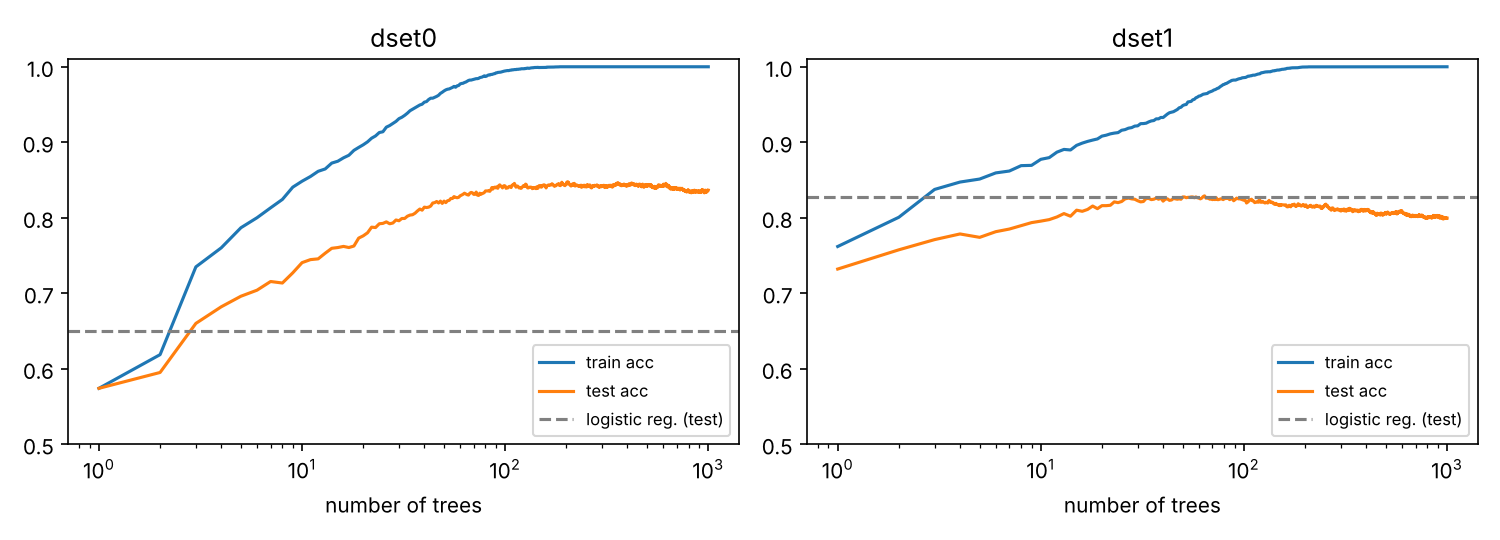
\includegraphics[width=.85\textwidth]{q3.png}
\end{center}

\textbf{(a) dset0.} Test accuracy rises steadily up to about 100--300 trees ($\approx.84$). From there through 1000 trees, test accuracy remains approximately stable ($.842\to.836$), even though training accuracy reaches $100\%$. Test log-loss, however, rises after about 100 trees, because the predicted probabilities become overconfident.

\textbf{(b) dset1.} Test accuracy peaks earlier, around 100 trees ($.824$), and then declines to $.799$ at 1000 trees, as the model interpolates the training data. Test log-loss worsens sharply ($.39\to.95$). At the evaluated tree counts, boosting does not outperform logistic regression ($.828$). Here the number of trees acts as a regularization parameter, and early stopping helps.

\textbf{(c)} The behaviour differs mainly in test accuracy; on both datasets, log-loss eventually overfits. A plausible explanation is that the two datasets differ in how complex the signal is relative to the noise:
\begin{itemize}[nosep]
\item \emph{dset0} appears to have a nonlinear signal involving interactions. Logistic regression reaches only $.65$, while boosting reaches $.84$. The additional trees keep learning real structure, so accuracy holds up even after the model fits the training data perfectly.
\item \emph{dset1} appears to have a simpler, near-linear decision boundary. Logistic regression ($.83$) matches boosting, and $x_1$ alone is strongly predictive. Once the boundary has been learned, later trees are likely fitting label noise or spurious feature patterns, so test accuracy declines.
\end{itemize}
This interpretation is consistent with the observations, but it is not a proof of the data-generating mechanism.

\end{document}
